% ----------------------------------------------------------
% Desenvolvimento
% ----------------------------------------------------------
\chapter{Desenvolvimento}
\label{cap:desenvolvimento}
% ----------------------------------------------------------
Neste capítulo, serão apresentados os elementos fundamentais envolvidos na criação da plataforma de artistas para a Casa de Cultura de João Monlevade. Serão discutidos aspectos gerais do sistema, com foco na sua arquitetura, nas tecnologias escolhidas para sua implementação, nas funcionalidades oferecidas aos usuários e nos principais artefatos gerados durante o processo de desenvolvimento.

Para a modelagem e estruturação do sistema, foram utilizados os conceitos da UML, uma linguagem padrão na modelagem de software. Entre os diagramas elaborados estão o diagrama de classes, que mapeia a estrutura das entidades do sistema, e o diagrama de casos de uso, que descreve como os usuários interagem com as funcionalidades. Além disso, foi desenvolvido um diagrama entidade-relacionamento, destacando as relações entre as diferentes entidades do banco de dados, garantindo uma visão clara da organização e fluxo das informações dos artistas.

\section{Modelo Conceitual}

O modelo conceitual proposto para o desenvolvimento do site web da Casa de Cultura de João Monlevade é estruturado para atender às necessidades específicas da instituição e da comunidade, proporcionando uma plataforma digital funcional, intuitiva e centrada na valorização da cultura local.

\subsection{Estrutura Geral do Site}

O site será organizado em uma arquitetura clara e acessível, com navegação intuitiva para garantir uma experiência de usuário fluida. A estrutura básica incluirá as seguintes seções:

Página Inicial: Um portal de entrada visualmente simples e elegante, destacando as principais atividades, eventos e notícias da Casa de Cultura. A página inicial funcionará como um resumo dinâmico do que está acontecendo na instituição, com links diretos para as seções e notícias mais relevantes.

Vitrine de Artistas: Uma seção dedicada à promoção dos talentos locais, onde artistas podem exibir suas obras, biografias, e links para suas redes sociais ou portfólios. Esta seção será categorizada por áreas de atuação, como artes plásticas, música, dança, e literatura, permitindo uma navegação fácil e segmentada. A inclusão de artistas na vitrine será gerenciada pela Casa de Cultura.

Editais e Inscrições: Um espaço para a publicação de editais e abertura de inscrições para eventos, cursos e concursos promovidos pela Casa de Cultura. Esta seção incluirá funcionalidades para que os interessados possam se inscrever online, acompanhar o status de suas inscrições e acessar documentos relevantes.

Escola de Artes: Uma área específica para a Escola de Artes, com informações sobre os cursos oferecidos, horários, e formas de inscrição. Essa seção também permitirá o acesso de alunos e responsáveis, permitindo a visualização de informações relevantes como notas e ocorrências.

Agenda de Eventos: Um calendário interativo que permitirá aos usuários acompanhar os próximos eventos culturais promovidos pela Casa de Cultura. A agenda será integrada com a Vitrine de Artistas e outras seções do site, facilitando a navegação e o acesso à informação.

Sobre Nós: Uma seção institucional com informações sobre a história, missão, e equipe da Casa de Cultura, além de um canal de contato direto com a instituição.

\subsection{Funcionalidades e Recursos}

Para garantir que o site atenda aos objetivos definidos, o modelo conceitual inclui as seguintes funcionalidades:

Responsividade: O site será completamente responsivo, adaptando-se automaticamente a diferentes dispositivos e tamanhos de tela, garantindo uma experiência de usuário consistente em desktops, tablets, e smartphones.

Sistema de Gerenciamento de Conteúdo \ac{CMS}: O backend do site será desenvolvido utilizando um sistema de gerenciamento de conteúdo, o Wagtail CRX baseado em Wagtail, para facilitar a atualização de informações e a adição de novos conteúdos sem a necessidade de conhecimentos técnicos avançados. Isso ajudará aos colaboradores a utilizar o sistema.

Sistema de Gestão da Casa de Cultura: Juntamente com o site, será desenvolvido utilizando a ferramenta Django admin a parte administrativa para utilização dos colaboradores da casa de cultura. A principio, essa seção posibilitará o acompanhamento dos editais, envolvendo sua criação, publicação e aprovação do público inscrito. Também será possível acessar informações sobre a Escola de Artes e a criação/edição de turmas, alunos, professores. A Vitrine de Artistas também será modificável através desse meio.

Segurança e Privacidade: O modelo prevê a implementação de boas práticas de segurança digital, garantindo a proteção dos dados dos usuários e a conformidade com a legislação vigente sobre proteção de dados.

\subsection{Fluxos de Usuário}

O modelo conceitual também define os principais fluxos de usuário, como:

Interação e Navegação: Usuários poderão acessar rapidamente as informações desejadas por meio de um menu de navegação simples e intuitivo, além de uma barra de busca eficiente.

Inscrição e Participação em editais: Processos de inscrição em eventos, cursos e editais serão simplificados, permitindo que os usuários visualizem os editais vigentes e passados, preencham formulários online e recebam confirmações e atualizações diretamente pelo site.

Visualização da Vitrine de Artistas: Poderá ser acessada através de um botão no menu de navegação para fácil acesso da comunidade.

Acesso à Escola de Artes: Haverá um link no menu de navegação para o redirecionamente à seção da escola.

Este modelo conceitual foi desenvolvido para garantir que o site da Casa de Cultura de João Monlevade não apenas atenda às necessidades atuais da instituição, mas também seja escalável e adaptável a futuras demandas, proporcionando uma plataforma duradoura e de valor para a comunidade.

\section{Funcionalidades do site}
%------------------------------------
%Funcionalidades do site web: ................................................................. 06-08
%Vitrine para artistas locais: Cadastro de artistas; Criação de perfis;
%Publicação de portfólios; Agenda de eventos.
%Controle de editais: Publicação de editais; Inscrições para editais;
%Seleção de projetos;
%Diário de classe e controle de alunos: Cadastro de alunos; Frequência;
%Histórico escolar.
%------------------------------------

O site web desenvolvido para a Casa de Cultura de João Monlevade foi projetado para oferecer uma diversa gama de funcionalidades que atendem tanto às necessidades da instituição quanto à comunidade local. Essas funcionalidades foram organizadas em três principais áreas: Vitrine para Artistas Locais, Controle de Editais e Controle da Escola de Artes.

\subsection{Página principal}

Inicialmente, foi considerado o uso de um bloco de carrossel para destacar as notícias mais relevantes no momento. Após analisar que o carrossel padrão do Wagtail CRX não atenderia às expectativas da casa de cultura, ficou decidido usar um outro carrossel bem popular atualmente. Assim, adaptou-se o template padrão do Wagtail CRX para utilizar o SlickSlider, um plugin de carrossel jQuery, integrando-o diretamente com a estrutura do Wagtail que gerencia o backend do site.

Para permitir a utilização do SlickSlider no projeto, foi necessário alterar o template do carrossel padrão. Dessa forma, o bloco continua registrado no admin do Wagtail, permitindo que ele possa ser escolhido e configurado diretamente na interface de gerenciamento de conteúdo, com as mesmas funcionalidades do carrossel padrão do Wagtail CRX.

O código do template foi colocado no arquivo carousel\_block.html, dentro da pasta templates, ficando assim configurado para renderizar o slider nas páginas onde ele fosse adicionado. Isso permitiu uma maior flexibilidade na personalização das páginas da Casa de Cultura, garantindo que o layout possa ser ajustado de acordo com a necessidade, conforme pode ser visto na \autoref{fig_pagina_principal}.

\begin{figure}[htb]
	\caption{\label{fig_pagina_principal}Página principal}
	\begin{center}
	    
\includegraphics[scale=0.35]{./img/pagina_principal.png}
	\end{center}
	\legend{Fonte: o autor}
\end{figure}


\subsection{Vitrine para Artistas Locais}

Uma das funcionalidades centrais do site é a Vitrine para Artistas Locais, que oferece um espaço dedicado para que os artistas de João Monlevade possam se cadastrar e divulgar seus trabalhos. Essa seção inclui as seguintes funcionalidades:

Cadastro de Artistas: Os artistas podem se registrar no site, fornecendo informações básicas como nome, nome artístico, área de atuação, e links para suas redes sociais ou portfólios online. Essa funcionalidade foi planejada para ser simples e acessível, permitindo que artistas com diferentes níveis de familiaridade com tecnologia possam se inscrever.

Exibição dos Perfis: Após o cadastro, cada artista passa a ter um perfil dedicado no site, onde são exibidas informações relevantes sobre o mesmo como seu nome artístico, área de atuação, e categoria. Esses perfis servem como cartões de visita digitais, oferecendo uma plataforma centralizada para que os artistas se conectem com o público. A exibição dos perfis dos artistas depende da aprovação do gestor do site da Casa de Cultura.

Gerenciamento dos Artistas: Após o cadastro, as informações do artista ficam armazenadas no banco de dados do sistema de gestão. O gestor do site será o responsável por aprovar ou não a exibição dos dados na página web da Casa de Cultura.

A criação da Vitrine de Artistas no website da Casa de Cultura de João Monlevade foi um processo que envolveu várias etapas de planejamento, implementação e integração com as ferramentas disponíveis no Wagtail CRX, que foi utilizado como base para o desenvolvimento do site.


\subsubsection{Interface do Django admin}

Para facilitar a gestão dos artistas cadastrados, foi criado um seção no Django admin personalizado para a Vitrine de Artistas. Isso permitiu que administradores do site pudessem facilmente adicionar, editar e remover artistas, além de gerenciar suas informações de forma centralizada.

O Django admin foi configurado para exibir as informações dos artistas em um layout claro e organizado, com filtros por categorias e áreas de atuação, conforme pode ser visto na \autoref{fig_adm_vitrine}. Também foram adicionadas funcionalidades para facilitar a busca e a edição em massa de registros.

\begin{figure}[htb]
	\caption{\label{fig_adm_vitrine}Página de administração da Vitrine de Artistas}
	\begin{center}
	    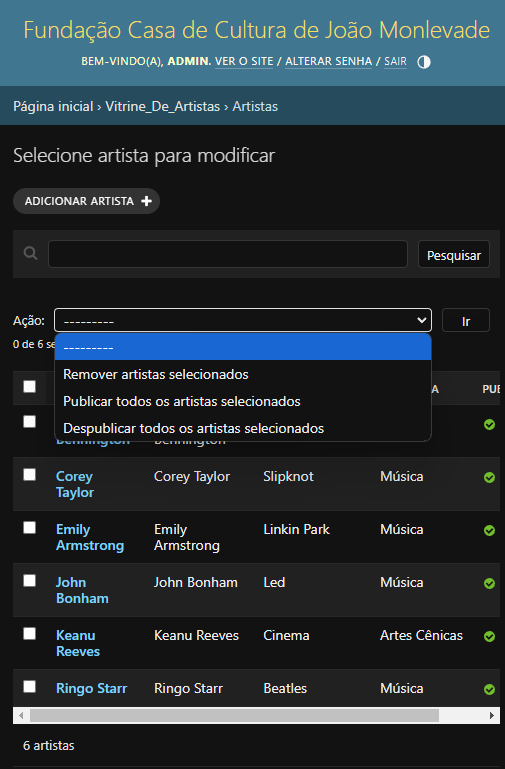
\includegraphics[scale=0.45]{./img/admin_artista.png}
	\end{center}
	\legend{Fonte: o autor}
\end{figure}

\subsubsection{Exibição dos Artistas no Website}

Para a exibição dos artistas no website, foi necessário desenvolver um layout utilizando Bootstrap. O objetivo foi criar uma apresentação visual atraente e funcional, onde cada artista seria exibido em um card. Esses cards devem ser responsivos e garantir que as imagens dos artistas sejam redimensionadas corretamente, mantendo um formato quadrado e destacando a imagem sobre o texto.

A implementação envolveu o uso de grids de cards do Bootstrap, ajustados para exibir corretamente a categoria e a área de atuação no formato "categoria - área de atuação". O foco foi manter o layout limpo e moderno, garantindo que o conteúdo fosse acessível e atrativo para os usuários (\autoref{fig_vitrine}).

\begin{figure}[htb]
	\caption{\label{fig_vitrine}Página da Vitrine de Artistas}
	\begin{center}
	    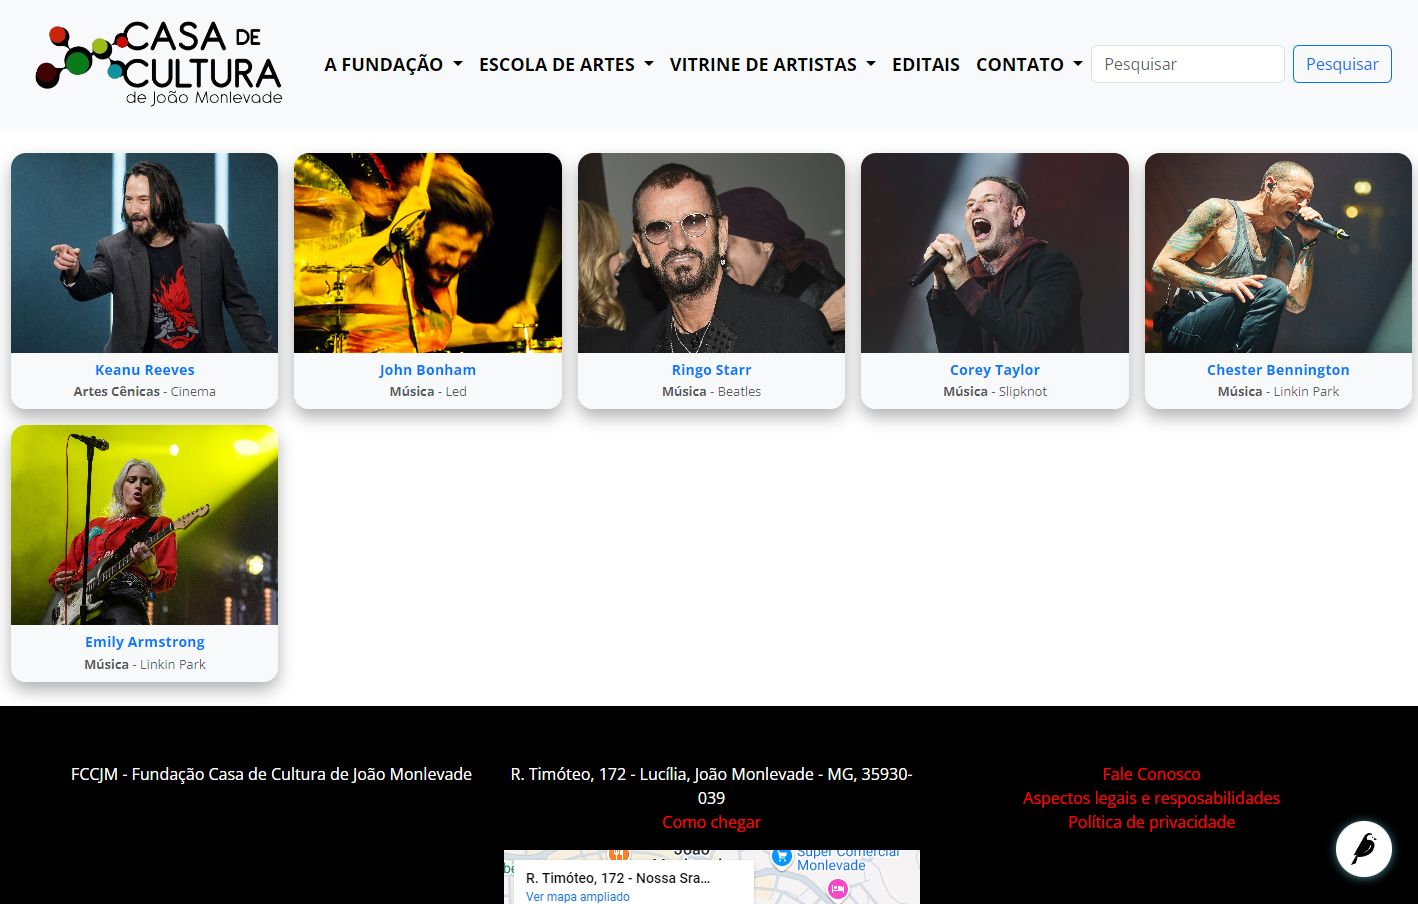
\includegraphics[scale=0.35]{./img/vitrine_de_artistas.png}
	\end{center}
	\legend{Fonte: o autor}
\end{figure}

Para melhorar a interatividade da Vitrine de Artistas, foi implementado um sistema onde o card inteiro seria clicável, redirecionando o usuário para uma página com mais detalhes sobre o artista selecionado. Isso foi feito utilizando \ac{HTML} padrão e funcionalidades nativas do Bootstrap, sem a necessidade de \ac{CSS} personalizado.


\begin{figure}[htb]
	\caption{\label{fig_grafico}Efeito flutuante}
	\begin{center}
	    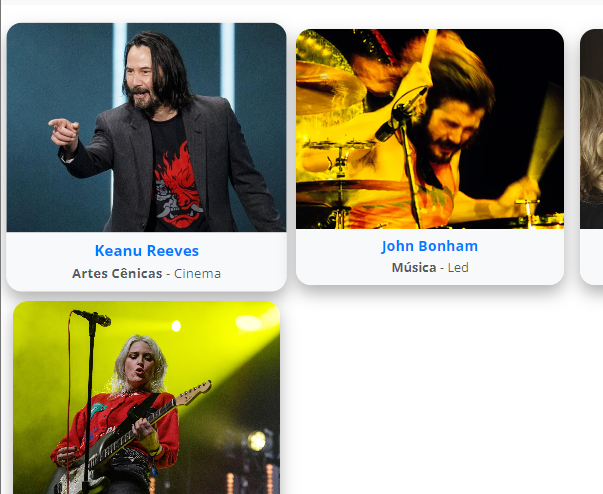
\includegraphics[scale=0.5]{./img/vitrine_de_artistas_hover.png}
	\end{center}
	\legend{Fonte: o autor}
\end{figure}

Com a implementação da Vitrine de Artistas, o website da Casa de Cultura de João Monlevade passa a contar com uma plataforma robusta para a divulgação dos artistas locais. A utilização de tecnologias como Django, Wagtail e Bootstrap permitiu a criação de um sistema que combina funcionalidade e estética, proporcionando uma experiência de usuário agradável e intuitiva.

Essa solução não apenas facilita a gestão e a exibição dos artistas, mas também fortalece a presença digital da Casa de Cultura, oferecendo um espaço dedicado para que os talentos locais possam ser devidamente reconhecidos e acessados pela comunidade.

\subsection{Escola de Artes}

O desenvolvimento do sistema de gestão para a Escola de Artes no website da Casa de Cultura de João Monlevade foi uma tarefa que envolveu a criação de modelos personalizados, integrações com o Django admin, e a implementação de funcionalidades que visavam facilitar o gerenciamento de alunos, turmas e professores, além de permitir o acesso controlado a dados específicos.

\subsubsection{Interface do Django admin}

A gestão desses modelos foi centralizada no Django admin, com uma interface personalizada para facilitar a administração de todos os dados relacionados à Escola de Artes. A configuração do Django admin foi feita de maneira a permitir uma visualização clara e organizada dos registros de alunos, professores e turmas.

Além disso, foi implementado um sistema que permitia a criação de usuários no momento do cadastro dos alunos. Esses usuários poderiam ser responsáveis (no caso de dependentes) ou os próprios alunos. A funcionalidade de geração de links para configuração de login e senha foi integrada, garantindo que cada usuário pudesse definir suas credenciais de acesso de maneira segura e eficiente.

Um dos desafios enfrentados foi o controle de acesso às informações de alunos e turmas. O sistema foi configurado para garantir que cada usuário, ao logar no site, só pudesse visualizar os dados referentes a si mesmo ou aos alunos sob sua responsabilidade.

Essa funcionalidade foi implementada utilizando as ferramentas nativas do Django para controle de permissões, onde cada usuário tinha seu acesso limitado aos dados específicos com base em seu papel (aluno ou responsável). Esse controle foi estendido para o Diário de Classe, garantindo que os registros fossem mantidos privados e acessíveis apenas aos professores responsáveis e aos administradores do sistema.

\begin{figure}[htb]
	\caption{\label{fig_grafico}Acesso do professor}
	\begin{center}
	    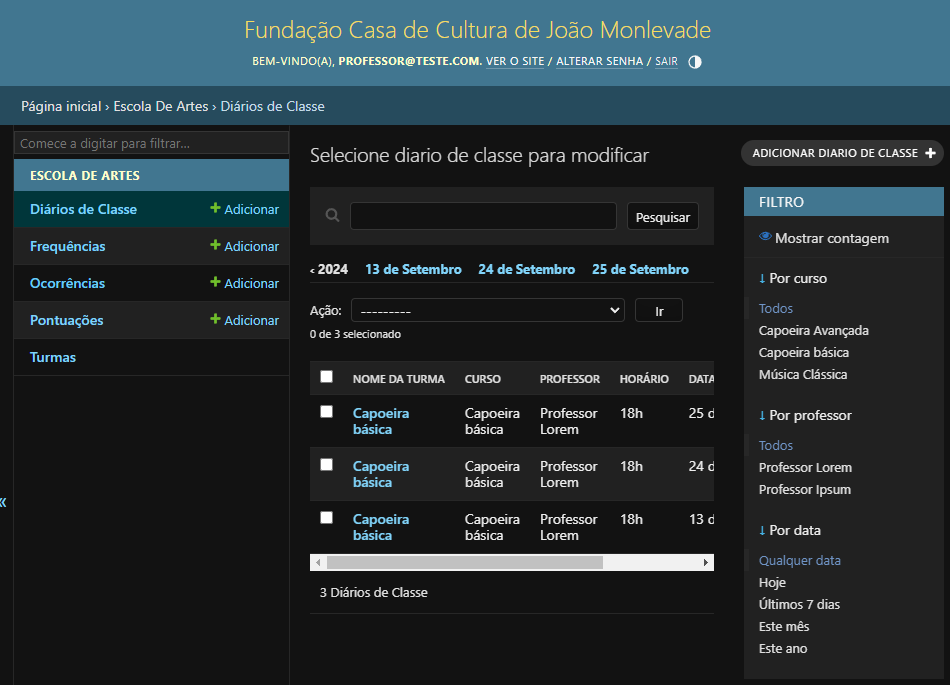
\includegraphics[scale=0.5]{./img/admin_professor.png}
	\end{center}
	\legend{Fonte: o autor}
\end{figure}

\subsubsection{Exibição de vagas no site}

O desenvolvimento do sistema de gestão da Escola de Artes traz diversas melhorias operacionais e administrativas para a Casa de Cultura de João Monlevade. A centralização dos dados e o controle de acesso eficiente permite que a administração da escola seja realizada de forma mais organizada e segura, garantindo a privacidade e a integridade dos dados dos alunos.

Outro processo que agora foi melhorado é o de inscrição em turmas. Acessando uma página dedicada no site, o usuário pode visualizar as turmas que estão com inscrições abertas e se inscrever através do próprio site, através de um formulário simplificado. Isso foi possível apartir da construção de um template de página específico para essa funcionalidade, que também foi reutilizado em outra parte do sistema, a de editais.

\begin{figure}[htb]
	\caption{\label{fig_grafico}Lista de vagas disponíveis}
	\begin{center}
	    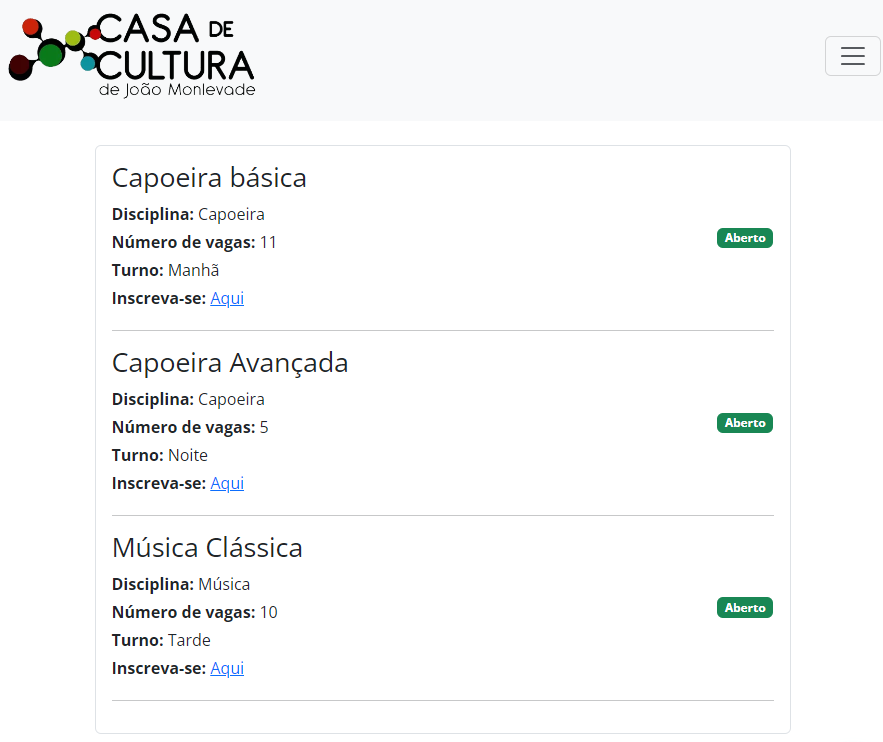
\includegraphics[scale=0.5]{./img/lista_turmas.png}
	\end{center}
	\legend{Fonte: o autor}
\end{figure}

A integração com o Django admin e o sistema de inscrições online também facilita o processo de matrícula e acompanhamento dos alunos, oferecendo uma plataforma moderna e intuitiva tanto para os administradores quanto para os usuários finais.

\subsection{Controle de Editais}

Outra funcionalidade essencial do site é o Controle de Editais, voltado para a gestão de processos seletivos e concursos promovidos pela Casa de Cultura. As funcionalidades nessa área incluem:

Publicação de Editais: A Casa de Cultura pode publicar editais diretamente no site, com informações detalhadas sobre prazos, requisitos, e critérios de seleção. Cada edital terá uma página específica onde os interessados podem acessar todos os detalhes necessários para a inscrição.

Inscrições para Editais: Os usuários do site podem se inscrever nos editais diretamente pela plataforma. A funcionalidade inclui a possibilidade de preenchimento de formulários online e upload de documentos exigidos, facilitando o processo de inscrição e garantindo que todas as submissões sejam centralizadas.

Gerenciamento dos Editais: Também após a inscrição, as informações do candidato ficam salvas no banco de dados do sistema de gestão. Apartir disso, a Casa de Cultura poderá aprovar ou nao sua candidatura à aquele edital.

\subsubsection{Interface do Django admin}

A gestão desses modelos também foi adicionada no Django admin, com uma interface personalizada para facilitar a administração dos dados relacionados aos editais. A configuração do Django admin foi feita de maneira a permitir uma visualização clara e organizada das candidaturas e editais publicados.

Através da página administrativa, o funcionário da casa de cultura poderá visualizar, criar, editar e deletar novos ou presentes editais, além de aprovar ou não candidaturas a estes. Também é possível visualizar todos os documentos referentes aos editais, tanto da sua publicação quanto dos candidatos. Também foram criados filtros que melhoram a usabilidade da ferramenta.

\begin{figure}[htb]
	\caption{\label{fig_grafico}Página administrativa dos editais}
	\begin{center}
	    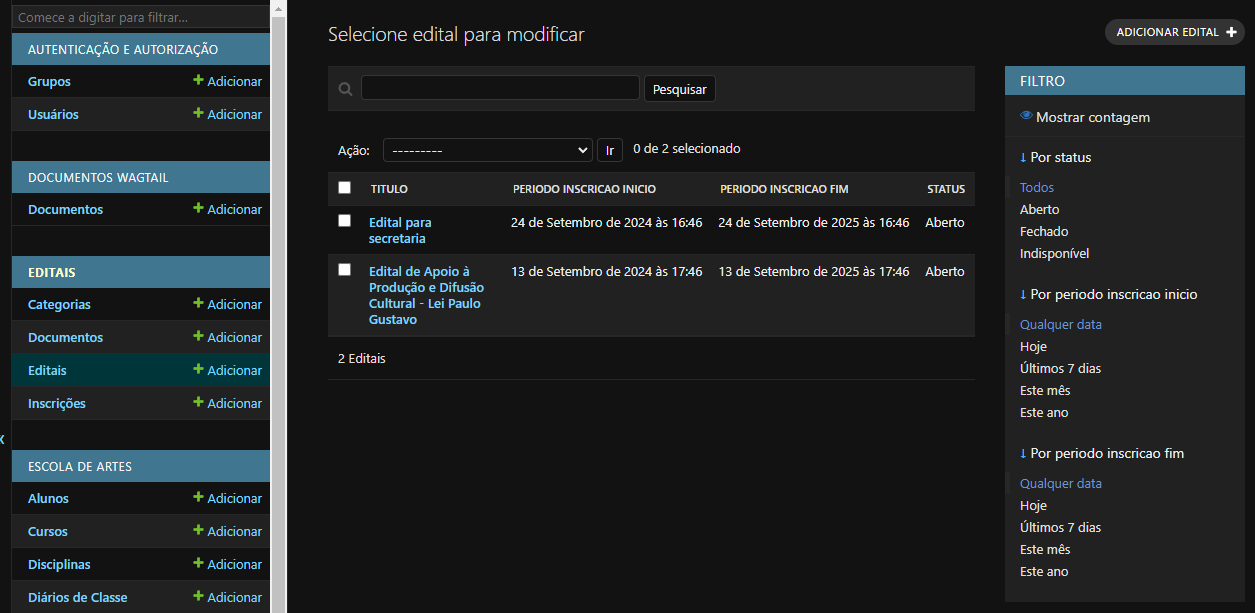
\includegraphics[scale=0.45]{./img/admin_edital.png}
	\end{center}
	\legend{Fonte: o autor}
\end{figure}


Um dos desafios enfrentados foi justamente o gerenciamento de múltiplos documentos que poderiam ser anexados em um formulário de candidatura. O sistema foi configurado para garantir que cada candidatura tivesse um relacionamento muitos-para-muitos com a classe Documentos, resolvendo assim essa questão.

\subsubsection{Exibição de editais no site}

Similarmente a Escola de Artes, a seção de editais no site da Casa de Cultura surge como uma grande ferramenta para os processos administrativos, também mostrando-se de extrema importância para a população, que poderá ter o acesso aos status dos editais publicados pela fundação.

Em uma página própria, o usuário poderá ver todos os editais já publicados e aqueles que estão abertos, os quais poderá se canditadar através do próprio site.

\begin{figure}[htb]
	\caption{\label{fig_grafico}Lista de editais}
	\begin{center}
	    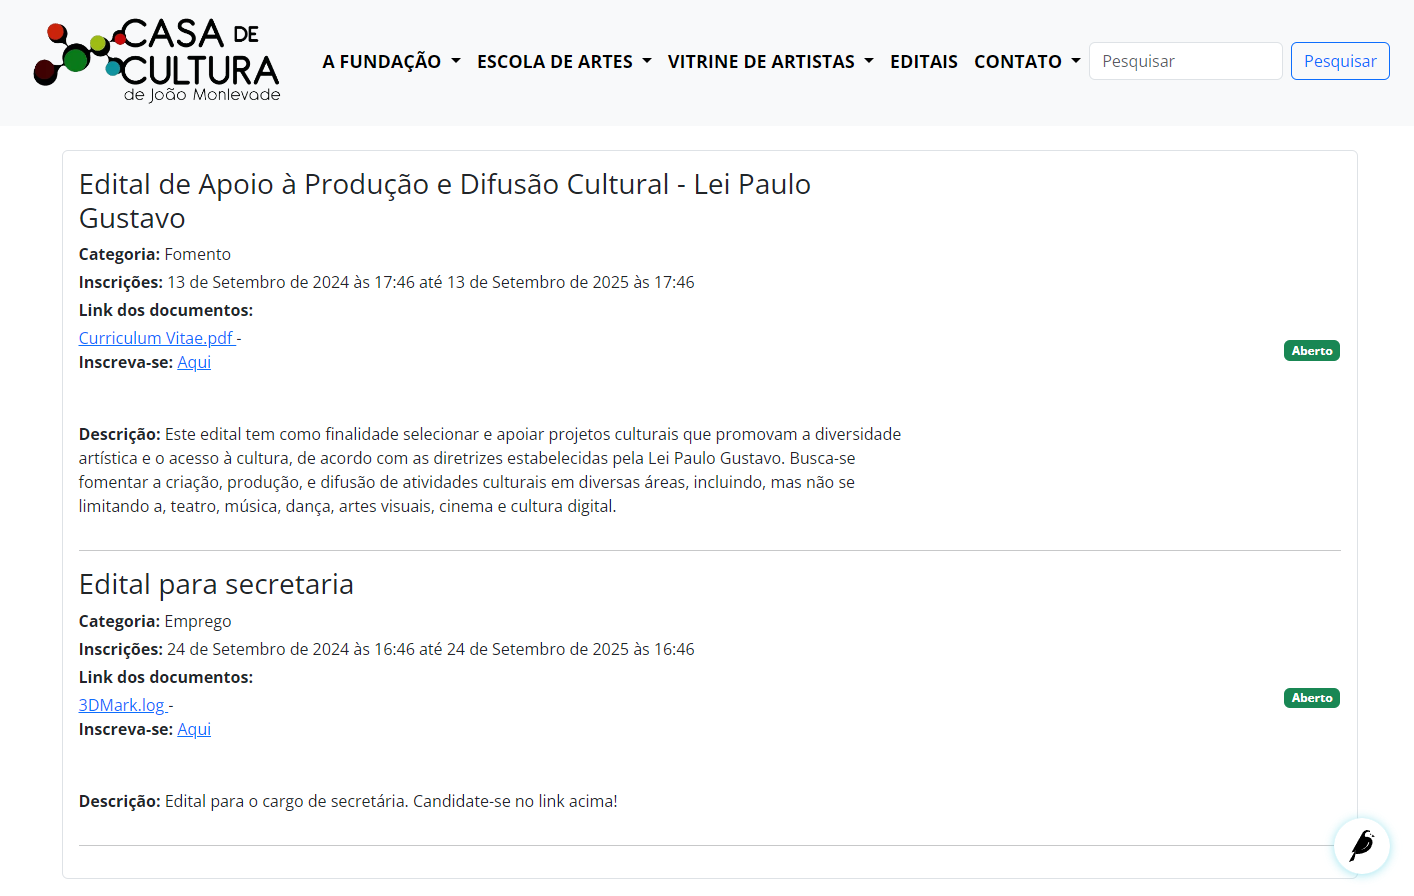
\includegraphics[scale=0.35]{./img/lista_editais.png}
	\end{center}
	\legend{Fonte: o autor}
\end{figure}

A integração com o Django admin e o sistema de inscrições online também facilita o processo de matrícula e acompanhamento dos alunos, oferecendo uma plataforma moderna e intuitiva tanto para os administradores quanto para os usuários finais. A inscrição através de um formulário simplificado no site torna a experiência simples e agradável.

\begin{figure}[htb]
	\caption{\label{fig_grafico}Formulário de um edital}
	\begin{center}
	    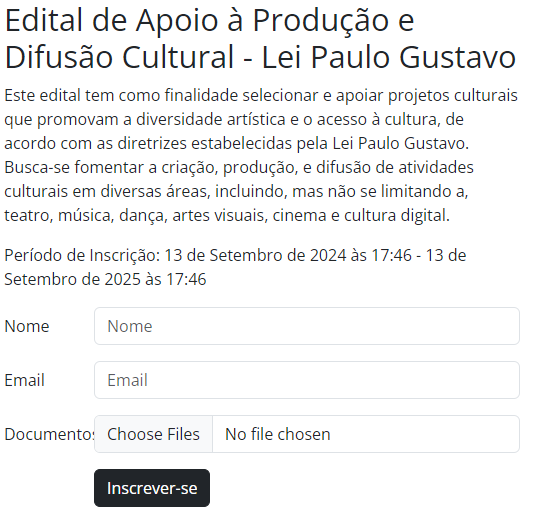
\includegraphics[scale=0.3]{./img/form_edital.png}
	\end{center}
	\legend{Fonte: o autor}
\end{figure}

\section{Arquitetura do Site Web}

A arquitetura de um site web, especialmente no que se refere ao layout e design, desempenha um papel crucial na criação de uma experiência de usuário eficiente e visualmente impactante. Um layout bem estruturado organiza os elementos da página de forma lógica e acessível, facilitando a navegação e a busca por informações essenciais. Além disso, o design responsivo é fundamental para garantir que o site seja visualmente atraente e funcional em diversos dispositivos, promovendo uma interface adaptável que atenda às necessidades dos usuários em diferentes contextos de uso \cite{garrett2010elements}. A escolha criteriosa da paleta de cores, tipografia e hierarquia visual não só reforça a identidade da marca, mas também guia o usuário de maneira intuitiva através do conteúdo, estabelecendo uma conexão emocional que melhora a usabilidade e fortalece a credibilidade do site.

\subsection{Layout e Design}

No desenvolvimento do site da Casa de Cultura de João Monlevade, utilizando o Wagtail CRX, o layout e o design foram estrategicamente pensados para proporcionar uma experiência de usuário que fosse simultaneamente fluida e esteticamente agradável, mantendo um equilíbrio entre simplicidade e sofisticação. Através da utilização de templates personalizados, suportados pelo Bootstrap, foi possível assegurar uma estrutura responsiva e coerente em todas as páginas, adaptando-se eficientemente a diferentes dispositivos, conforme preconizado por \citeonline{liddle2013design}. O design foi cuidadosamente planejado para refletir a rica identidade cultural da instituição, utilizando uma paleta de cores e uma tipografia que evocam tanto a tradição quanto a modernidade, alinhando-se perfeitamente ao propósito da Casa de Cultura. A organização do conteúdo segue uma hierarquia clara e intuitiva, facilitando a navegação e destacando informações cruciais como notícias culturais, acesso a subsistemas como editais, a vitrine de artistas e a Escola de Artes. Essa integração harmoniosa entre layout e design não só enriquece a usabilidade, mas também fortalece a conexão emocional dos visitantes com o site, criando um ambiente digital que é tanto acolhedor quanto representativo da riqueza cultural de João Monlevade.

\subsection{Navegação}

A navegação do site da Casa de Cultura de João Monlevade foi projetada para ser intuitiva e eficiente, assegurando que os usuários encontrem rapidamente as informações desejadas. A estrutura do site é organizada por meio de uma navbar que dispõe os principais menus de forma clara, facilitando o acesso a seções como "A fundação", "Contato" e "Vitrine de Artistas". As notícias, categorizadas de maneira lógica, permitem uma busca simplificada e mantêm o usuário engajado com o conteúdo \cite{nielsen2012usability}. 

Além disso, a integração de outros sistemas, como o da Escola de Artes, diretamente no site principal, onde também são publicados os editais, oferece uma experiência de usuário coesa e centralizada. Para garantir uma gestão séria e segura das informações, o acesso dos pais às ocorrências dos alunos é realizado exclusivamente através do Django admin, proporcionando um ambiente profissional e controlado. Essa abordagem de navegação não só aprimora a acessibilidade, mas também reforça a confiança dos usuários no sistema, refletindo o compromisso da instituição com a seriedade e transparência na gestão das informações.

\subsection{Tecnologias Utilizadas}

O desenvolvimento do site da Casa de Cultura de João Monlevade envolveu a aplicação de tecnologias robustas, com destaque para o Wagtail CRX, uma plataforma baseada em Django que facilita a criação e gestão de conteúdo. Este \ac{CMS} oferece funcionalidades padrão, como gestão de páginas, formulários, menus dinâmicos e integração com diversos módulos, permitindo uma customização extensiva dos templates para atender às necessidades específicas do site \cite{ellis2015coders}. Bootstrap, amplamente utilizado no projeto, é essencial para garantir que a navegação seja responsiva e consistente em todos os dispositivos, graças aos seus componentes pré-construídos, como navbar, dropdowns e sistemas de grid, que tornam o desenvolvimento mais ágil e uniforme. 

A capacidade de personalização oferecida pelos templates do Django permite que cada detalhe do layout e da navegação seja ajustado para refletir com precisão a identidade visual da Casa de Cultura, resultando em uma experiência de usuário intuitiva e envolvente. A combinação dessas tecnologias proporciona um site funcional, esteticamente atraente e fácil de navegar, contribuindo para uma presença digital impactante e eficaz.

Para a customização do carrossel padrão do Wagtail CRX, foi implementado o SlickSlider, modificando o template do mesmo. A Vitrine de Artistas também utiliza um template, por sua vez, desenvolvido pelo autor para este uso específico usando Bootstrap e \ac{CSS}. Outras seções que utilzaram templates foram a listagem de editais e de turmas disponíveis.

\section{Banco de Dados}

A estrutura de um banco de dados, fundamental para qualquer aplicação web, define a forma como os dados são organizados e armazenados. Modelos de dados relacionais, como o MySQL, PostgreeSQL e SQL Server são amplamente utilizados devido à sua flexibilidade e capacidade de representar complexas relações entre entidades. A integração desses bancos com sites web é realizada através de linguagens de programação como PHP ou Python, que permitem a conexão, consulta e manipulação dos dados. A escolha do modelo de dados e a forma de integração devem considerar fatores como o volume de dados, a frequência de acesso e as necessidades específicas da aplicação. É crucial que a estrutura do banco de dados seja bem projetada para garantir a eficiência, a integridade e a segurança dos dados.

\subsection{Estrutura do banco de dados}

\subsubsection{Vitrine de Artistas}

Inicialmente, foi necessário definir a estrutura de dados para a Vitrine de Artistas, considerando as necessidades de armazenamento e apresentação de informações sobre os artistas locais. Foram criados modelos no Django para representar esses dados de maneira organizada e eficiente. Cada artista poderia ter informações como Nome, Nome Artístico, Área de Atuação, Links para portfólios ou redes sociais, documentos, imagens e uma categorização por área de atuação.

\begin{figure}[htb]
	\caption{\label{fig_grafico}Diagrama ER da Vitrine de Artistas}
	\begin{center}
	    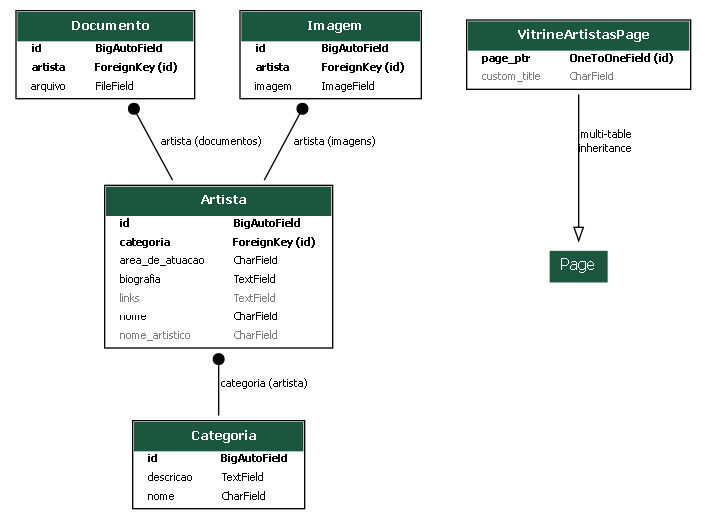
\includegraphics[scale=0.3]{./img/er_diagram_vitrine.png}
	\end{center}
	\legend{Fonte: o autor}
\end{figure}



\subsubsection{Escola de Artes}

O modelo de dados para a Escola de Artes é estruturado de forma a atender às diversas necessidades operacionais e acadêmicas da instituição. Este modelo é essencial para o gerenciamento eficaz dos cursos, alunos, responsáveis, professores, e outros aspectos relacionados ao bom funcionamento da escola.

A base do modelo é o Curso, que representa as disciplinas oferecidas pela escola. Cada curso é caracterizado pelo nome, disciplina, turno e número de vagas disponíveis. As disciplinas são definidas pelo modelo Disciplina, que pode incluir opções como Capoeira, Violão e Pintura e Desenho. O turno do curso pode ser Manhã, Tarde ou Noite, e o número de vagas é validado para garantir que se mantenha dentro de um intervalo apropriado.

As Turmas são associadas a um curso e a um professor, e podem ter vários alunos. Cada turma possui um nome e horário específicos, facilitando a organização das aulas e a alocação dos recursos.

Os Professores são representados com detalhes como nome, especialidade, e-mail e telefone. Eles são associados aos cursos através das turmas e têm uma relação de um-para-um com o modelo User do Django, permitindo o gerenciamento de suas credenciais de acesso.

O modelo de Aluno captura informações abrangentes sobre os estudantes, incluindo nome, CPF, RG, data de nascimento, e-mail, endereço e telefone. Os alunos podem ter documentos anexados e, caso sejam dependentes, são vinculados a responsáveis através de uma relação de um-para-um. Cada aluno também possui um link único para configurar o acesso ao sistema através do modelo User do Django com uma relação de um-para-um, caso ele não seja um dependente.

Os Responsáveis são os indivíduos que, muitas vezes, são os pais ou responsáveis legais dos alunos. Cada responsável possui informações detalhadas como nome, CPF, data de nascimento, e-mail, endereço e telefone. Além disso, o modelo inclui a capacidade de anexar documentos relevantes e gerar um link único para configurar o acesso ao sistema através do modelo User do Django, com uma relação de um-para-um. A associação de um responsável com um aluno é feita através do campo responsavel, permitindo apenas um responsável para cada aluno.

Para registrar ocorrências, acompanhar a frequência e a pontuação dos alunos, foram criados os modelos Ocorrência, Frequência e Pontuação. O modelo de Ocorrência documenta eventos específicos que afetam um aluno em um determinado dia, enquanto o modelo de Frequência rastreia a presença dos alunos e permite justificativas para ausências. A Pontuação avalia o desempenho dos alunos em diferentes aspectos, como assiduidade, comportamento e aptidão. Esses dados são críticos para monitorar o progresso dos alunos e identificar áreas que necessitam de atenção.

O Diário de Classe é um registro diário das atividades da turma. Cada entrada no diário está associada a uma turma específica e a uma data, proporcionando uma visão detalhada do progresso e das atividades da turma ao longo do tempo. A data do diário é adicionada automaticamente de acordo com o dia atual no momento da criação do diário, mas pode ser modificada caso seja necessário. Esse modelo agrupa as informações das ocorrências, frequência e pontuação para um determinado dia de aula.

Finalmente, o modelo de Inscrição registra as inscrições dos alunos em cursos específicos, incluindo observações adicionais e a data de inscrição. Este modelo garante que o processo de matrícula seja registrado de maneira estruturada e eficiente. Abaixo está descrito com mais detalhes o diagrama ER da Escola de artes.


\begin{figure}[htb]
	\caption{\label{fig_grafico}Diagrama ER da Escola de Artes}
	\begin{center}
	    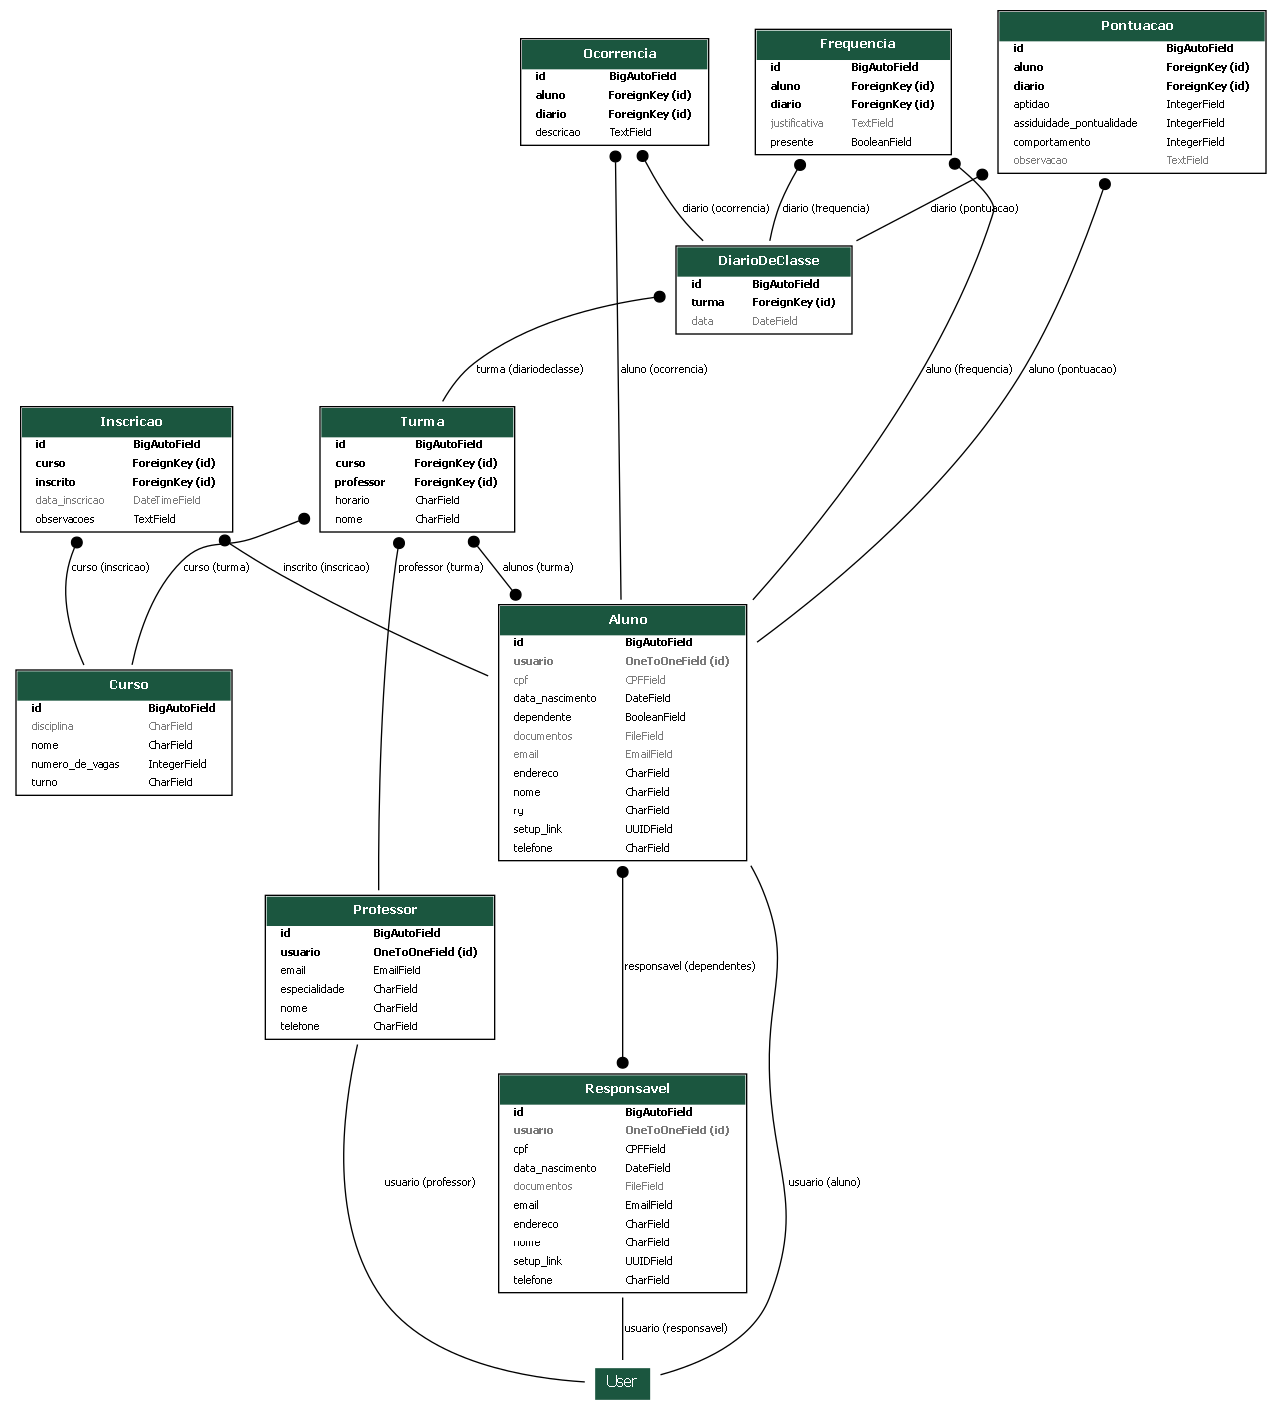
\includegraphics[scale=0.3]{./img/er_diagram_escola.png}
	\end{center}
	\legend{Fonte: o autor}
\end{figure}

\subsubsection{Editais}

O modelo de dados para a seção de Editais é crucial para a gestão e operacionalização de processos seletivos e inscrições dentro do sistema. Este conjunto de modelos foi desenvolvido para facilitar a criação, gerenciamento e inscrição em editais, bem como para a comunicação eficiente com os participantes.

O Edital é a entidade fundamental do sistema, representando um processo seletivo ou oportunidade de inscrição. Cada edital possui um título, uma descrição detalhada, uma categoria, um período de inscrição definido por uma data e hora de início e término, e um status que pode ser "Aberto", "Fechado" ou "Indisponível". O status do edital é dinamicamente atualizado através do método "atualizar\_status", que compara a data e hora atuais com o período de inscrição para determinar se o edital está aberto para novas inscrições. Caso o edital esteja fora do período de inscrição, seu status é atualizado para "Fechado".

O modelo de Inscrição é utilizado para registrar as inscrições de candidatos em editais específicos. Cada inscrição está associada a um edital e contém informações do candidato, como nome, e-mail e um documento de apoio. Além disso, a inscrição inclui um campo de protocolo único, gerado com base no ID do edital, ID do usuário e ID da própria inscrição. Esse protocolo é atribuído no momento da criação da inscrição. O modelo também possui um campo para marcar a aprovação da inscrição e, se aprovado, um e-mail de chamamento é enviado ao candidato, informando-o sobre sua aprovação.

A classe EditaisPage é uma página do Wagtail que exibe uma lista de editais disponíveis. Esta página usa um template para apresentar a lista de editais e permite personalizar o título da página. O método get\_context é usado para adicionar todos os editais ao contexto da página, garantindo que a lista mais atualizada de editais esteja disponível para visualização.

Similarmente, a EditailInscreverPage é uma página do Wagtail dedicada aos detalhes de um edital específico, permitindo que os usuários visualizem informações detalhadas sobre o edital e se inscrevam. Esta página também utiliza um template e permite a personalização do título. O método get\_context é utilizado para fornecer o contexto necessário, daquele edital específico.

Este conjunto de modelos fornece uma estrutura robusta para o gerenciamento de editais e inscrições, garantindo que as informações sejam mantidas de forma organizada e acessível. Além disso, as funcionalidades integradas de atualização de status e envio de e-mails ajudam a manter a comunicação fluida e eficiente com os participantes, enquanto as páginas do Wagtail oferecem uma interface amigável para a visualização e interação com os editais.

\begin{figure}[htb]
	\caption{\label{fig_grafico}Diagrama ER dos Editais}
	\begin{center}
	    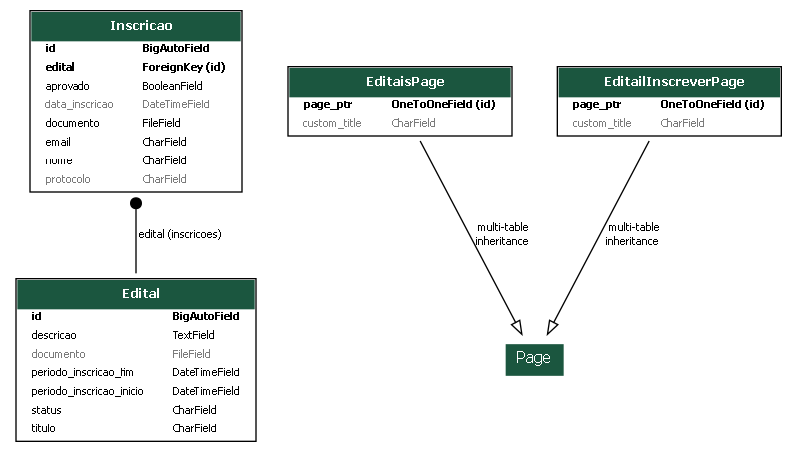
\includegraphics[scale=0.3]{./img/er_diagram_editais.png}
	\end{center}
	\legend{Fonte: o autor}
\end{figure}


\subsection{Integração com o site}

A plataforma desenvolvida para a Casa de Cultura de João Monlevade utiliza o SQLite3 como banco de dados principal nesta fase inicial do projeto. A escolha pelo SQLite3 foi motivada por sua simplicidade, eficiência e fácil integração com projetos de menor escala, como o atual. Esse banco de dados relacional armazena todas as informações em um único arquivo de disco, o que elimina a necessidade de um servidor dedicado, simplificando tanto a configuração quanto a manutenção do ambiente de desenvolvimento.

O SQLite3 oferece diversas vantagens, especialmente para protótipos e aplicações de pequeno porte. Sua leveza e facilidade de uso são fundamentais neste contexto, permitindo que o projeto avance sem a sobrecarga de gerenciar bancos de dados mais complexos. Além disso, o Django, framework utilizado no desenvolvimento do site, já traz o SQLite3 como banco de dados padrão, facilitando a integração com o Wagtail e o Wagtail CRX, ambos essenciais para a estrutura e gerenciamento de conteúdo da plataforma. A execução de migrações e modificações no banco de dados também se torna direta, aproveitando as ferramentas nativas do Django.

Apesar dos benefícios imediatos do SQLite3, é importante considerar que o projeto tem potencial para crescer, tanto em volume de dados quanto em complexidade. Nesse sentido, a plataforma foi projetada com a flexibilidade necessária para que, no futuro, o SQLite3 possa ser substituído por um banco de dados mais robusto, como PostgreSQL ou MySQL, com o mínimo de reestruturação. A transição entre esses sistemas é facilitada pelo uso de SQL como linguagem padrão em bancos relacionais, permitindo que alterações no código e na infraestrutura sejam feitas de maneira gradual e eficiente, conforme as necessidades da plataforma evoluam.